% Options for packages loaded elsewhere
% Options for packages loaded elsewhere
\PassOptionsToPackage{unicode}{hyperref}
\PassOptionsToPackage{hyphens}{url}
\PassOptionsToPackage{dvipsnames,svgnames,x11names}{xcolor}
%
\documentclass[
  11pt,
  letterpaper,
  DIV=11,
  numbers=noendperiod]{scrartcl}
\usepackage{xcolor}
\usepackage{amsmath,amssymb}
\setcounter{secnumdepth}{5}
\usepackage{iftex}
\ifPDFTeX
  \usepackage[T1]{fontenc}
  \usepackage[utf8]{inputenc}
  \usepackage{textcomp} % provide euro and other symbols
\else % if luatex or xetex
  \usepackage{unicode-math} % this also loads fontspec
  \defaultfontfeatures{Scale=MatchLowercase}
  \defaultfontfeatures[\rmfamily]{Ligatures=TeX,Scale=1}
\fi
\usepackage{lmodern}
\ifPDFTeX\else
  % xetex/luatex font selection
\fi
% Use upquote if available, for straight quotes in verbatim environments
\IfFileExists{upquote.sty}{\usepackage{upquote}}{}
\IfFileExists{microtype.sty}{% use microtype if available
  \usepackage[]{microtype}
  \UseMicrotypeSet[protrusion]{basicmath} % disable protrusion for tt fonts
}{}
% Make \paragraph and \subparagraph free-standing
\makeatletter
\ifx\paragraph\undefined\else
  \let\oldparagraph\paragraph
  \renewcommand{\paragraph}{
    \@ifstar
      \xxxParagraphStar
      \xxxParagraphNoStar
  }
  \newcommand{\xxxParagraphStar}[1]{\oldparagraph*{#1}\mbox{}}
  \newcommand{\xxxParagraphNoStar}[1]{\oldparagraph{#1}\mbox{}}
\fi
\ifx\subparagraph\undefined\else
  \let\oldsubparagraph\subparagraph
  \renewcommand{\subparagraph}{
    \@ifstar
      \xxxSubParagraphStar
      \xxxSubParagraphNoStar
  }
  \newcommand{\xxxSubParagraphStar}[1]{\oldsubparagraph*{#1}\mbox{}}
  \newcommand{\xxxSubParagraphNoStar}[1]{\oldsubparagraph{#1}\mbox{}}
\fi
\makeatother


\usepackage{longtable,booktabs,array}
\usepackage{calc} % for calculating minipage widths
% Correct order of tables after \paragraph or \subparagraph
\usepackage{etoolbox}
\makeatletter
\patchcmd\longtable{\par}{\if@noskipsec\mbox{}\fi\par}{}{}
\makeatother
% Allow footnotes in longtable head/foot
\IfFileExists{footnotehyper.sty}{\usepackage{footnotehyper}}{\usepackage{footnote}}
\makesavenoteenv{longtable}
\usepackage{graphicx}
\makeatletter
\newsavebox\pandoc@box
\newcommand*\pandocbounded[1]{% scales image to fit in text height/width
  \sbox\pandoc@box{#1}%
  \Gscale@div\@tempa{\textheight}{\dimexpr\ht\pandoc@box+\dp\pandoc@box\relax}%
  \Gscale@div\@tempb{\linewidth}{\wd\pandoc@box}%
  \ifdim\@tempb\p@<\@tempa\p@\let\@tempa\@tempb\fi% select the smaller of both
  \ifdim\@tempa\p@<\p@\scalebox{\@tempa}{\usebox\pandoc@box}%
  \else\usebox{\pandoc@box}%
  \fi%
}
% Set default figure placement to htbp
\def\fps@figure{htbp}
\makeatother





\setlength{\emergencystretch}{3em} % prevent overfull lines

\providecommand{\tightlist}{%
  \setlength{\itemsep}{0pt}\setlength{\parskip}{0pt}}



 


\usepackage{xcolor, soul}
\definecolor{Light}{gray}{.90}
\sethlcolor{Light}
\let\OldTexttt\texttt
\renewcommand{\texttt}[1]{\OldTexttt{\hl{#1}}}
\usepackage{caption}
\captionsetup{font=small, labelfont=bf}
\setlength{\parindent}{0pt}
\setlength{\parskip}{1.25ex}
\KOMAoption{captions}{tableheading}
\makeatletter
\@ifpackageloaded{caption}{}{\usepackage{caption}}
\AtBeginDocument{%
\ifdefined\contentsname
  \renewcommand*\contentsname{Table of contents}
\else
  \newcommand\contentsname{Table of contents}
\fi
\ifdefined\listfigurename
  \renewcommand*\listfigurename{List of Figures}
\else
  \newcommand\listfigurename{List of Figures}
\fi
\ifdefined\listtablename
  \renewcommand*\listtablename{List of Tables}
\else
  \newcommand\listtablename{List of Tables}
\fi
\ifdefined\figurename
  \renewcommand*\figurename{Figure}
\else
  \newcommand\figurename{Figure}
\fi
\ifdefined\tablename
  \renewcommand*\tablename{Table}
\else
  \newcommand\tablename{Table}
\fi
}
\@ifpackageloaded{float}{}{\usepackage{float}}
\floatstyle{ruled}
\@ifundefined{c@chapter}{\newfloat{codelisting}{h}{lop}}{\newfloat{codelisting}{h}{lop}[chapter]}
\floatname{codelisting}{Listing}
\newcommand*\listoflistings{\listof{codelisting}{List of Listings}}
\makeatother
\makeatletter
\makeatother
\makeatletter
\@ifpackageloaded{caption}{}{\usepackage{caption}}
\@ifpackageloaded{subcaption}{}{\usepackage{subcaption}}
\makeatother
\usepackage{bookmark}
\IfFileExists{xurl.sty}{\usepackage{xurl}}{} % add URL line breaks if available
\urlstyle{same}
\hypersetup{
  pdftitle={Inter-region sparsity initial results},
  pdfauthor={Al Xin},
  colorlinks=true,
  linkcolor={blue},
  filecolor={Maroon},
  citecolor={Blue},
  urlcolor={Blue},
  pdfcreator={LaTeX via pandoc}}


\title{Inter-region sparsity initial results}
\author{Al Xin}
\date{Oct 28, 2026}
\begin{document}
\maketitle


\section{Sparsity measures}\label{sparsity-measures}

\subsection{Lifetime vs.~population}\label{lifetime-vs.-population}

\subsection{Moment ratio}\label{moment-ratio}

A common lifetime sparsity measure is the ratio of moments (call this
the ``RM'' estimator) (Rolls and Tovee, 1995; Vinje and Gallant, 2000):
\[
S_{\textrm{RM}} = \left( 1 - \frac{\left( \frac{1}{n} \sum_{i = 1}^n r_i \right)^2}{\frac{1}{n} \sum_{i = 1}^n r_i^2} \right) \left( \frac{1}{1 - \frac{1}{n}} \right).
\] The term \(\left( \frac{1}{1 - \frac{1}{n}} \right)\) scales the
above to \([0, 1]\), with 0 indicating uniformity and 1 indicating
maximal concentration.

\subsection{Gini index}\label{gini-index}

Hurley and Rickard (2009) suggest the Gini coefficient (see also:
\texttt{DescTools::Gini()}). Assume that the rates are ordered as
\(r_{(1)}, r_{(2)}, \dots, r_{(n)}\). Then, \[
S_{\textrm{Gini}} = 
\frac{2}{n^2 \overline{r}}
\sum_{i = 1}^n i (r_{(i)} - \overline{r}), \quad \overline{r} = \frac{1}{n} \sum_{i = 1}^{n} r_i.
\] By default, the above falls within 0 and \(\sqrt{(n - 1) / n}\), so
dividing the above by \(\sqrt{(n - 1) / n}\) gives the same \([0, 1]\)
interpretation as the RM estimator.

\subsection{Entropy-based effective
dimensionality}\label{entropy-based-effective-dimensionality}

(Check this later).

\section{Data processing shifts
sparsity}\label{data-processing-shifts-sparsity}

Unless otherwise indicated, I will apply RM sparsity. In my initial
pass, the results did not change based on the sparsity metric.

\subsection{Baseline subtraction}\label{baseline-subtraction}

Unlike Mahalanobis distance, sparsity \emph{will} be affected by
shifting of the responses (but not scaling). In general, the addition of
a constant lowers the calculated sparsity (this is a known desirable
property of sparsity calculation). So, as an important processing
consideration, one might be interested in subtracting the baseline
response (mean response to blank stimuli). By subtracting the baseline,
one reports something that might be more interpretable as the sparseness
of the site response to stimuli.

For instance, let the baseline of a site be 60 Hz. If most of the
stimuli produce an average response of 61 Hz while a single stimulus
produces an average response of 80 Hz, the sparsity will look higher
after subtracting the baseline. The key question is: should this be
treated as the same sparsity as a site with a baseline of 0 Hz, most
stimuli evoking 1 Hz, and a single stimulus evoking 20 Hz? Furthermore,
what about a site with a baseline of 60 Hz, most stimuli evoking 59 Hz,
and a single stimulus at 40 Hz?

\begin{figure}

\centering{

\pandocbounded{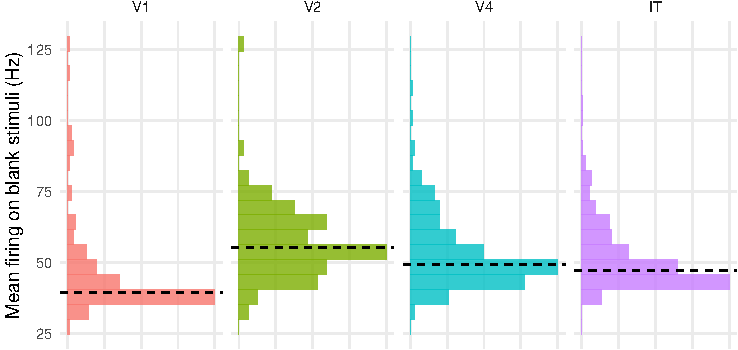
\includegraphics[keepaspectratio]{20261007_files/figure-pdf/fig-baselines-1.pdf}}

}

\caption{\label{fig-baselines}Histogram of per-site baseline firing
(mean response to blank image) for each region. Dashed lines indicate
medians.}

\end{figure}%

\subsubsection{Handling resulting
negatives}\label{handling-resulting-negatives}

As an additional concern, subtracting the baseline might yield a
negative number, which cannot be used in sparsity calculation. Let
\(\Delta r_i\) be the response minus the blank baseline. Truncating
negatives by taking \(\max(0, \Delta r_i)\) inflates the sparsity of
sites that are centered around the baseline. Taking the absolute value
after subtraction would deflate the sparsity of sites that tend to be
centered around the baseline (compared to truncating). (In practice, the
baseline subtraction makes sparsities net inflated)

\begin{figure}

\centering{

\pandocbounded{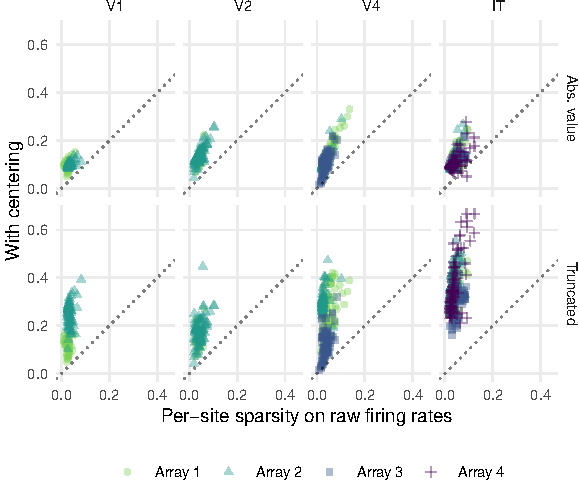
\includegraphics[keepaspectratio]{20261007_files/figure-pdf/fig-baseline-1.pdf}}

}

\caption{\label{fig-baseline}After subtracting the per-site mean
response to blank images, the calculated sparsity increases for each
site. Rows correspond to differnt approaches to handling negative
differences (Truncated: send to zero; Abs. value: take absolute value).
Sparsities calculated with RM on image-averaged responses.}

\end{figure}%

Figure~\ref{fig-baseline} shows the per-site sparsity shifts with these
different approaches. As expected, after subtracting the baseline, the
calculated sparsity increases. The shift with truncated negatives is
higher than with the absolute value.

\emph{If it can be justified}, I would prefer the baseline-centered
sparsity scores since the intuition more aligns with what I consider
``relevant'' sparsity. Also, the range appears wider and possibly more
informative. Interestingly, in the absolute value approach, V1 barely
shifts in sparsity.

\subsubsection{Relationship between sparsity changes and site
characteristics}\label{relationship-between-sparsity-changes-and-site-characteristics}

\begin{figure}

\centering{

\pandocbounded{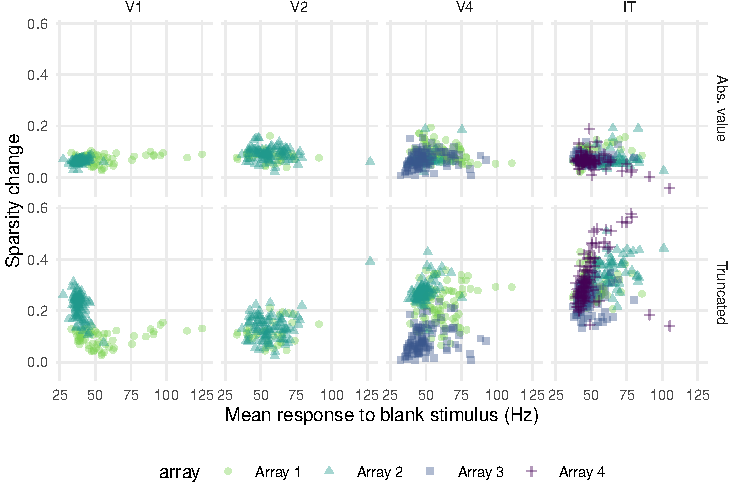
\includegraphics[keepaspectratio]{20261007_files/figure-pdf/fig-shift_vs_firing-1.pdf}}

}

\caption{\label{fig-shift_vs_firing}The baseline firing does not appear
related to the difference in sparsity except in IT, where they appear
somewhat positively correlated.}

\end{figure}%

Figure~\ref{fig-shift_vs_firing} shows that the change in calculated
sparsity with or without baseline centering does not appear to be
related to the baseline firing rate for V1, V2, and V4. However, when
truncating negatives, the relationship seems positive in IT.

\begin{figure}

\centering{

\pandocbounded{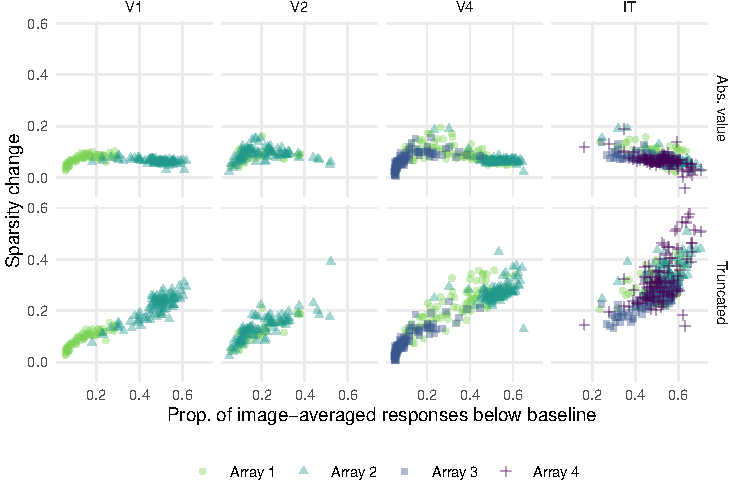
\includegraphics[keepaspectratio]{20261007_files/figure-pdf/fig-shift_vs_negatives-1.pdf}}

}

\caption{\label{fig-shift_vs_negatives}Truncating the zeroes produces a
marked inflation of the sparsity scores compared to taking the absolute
value.}

\end{figure}%

Figure~\ref{fig-shift_vs_negatives} shows the disadvantage of
truncation. When negatives are truncated to zero, the sites with the
most negatives show a positive relationship with the sparsity shift
(especially in IT). This relationship basically disappears when
negatives are taken as their absolute value.

\subsection{Effects of averaging on
sparsity}\label{effects-of-averaging-on-sparsity}

More averaging tends to decrease sparsity; this is expected based on the
removal of noise (Figure~\ref{fig-sparsity_avgs}). It seems most
``sane'' to perform image-averaged sparsity calculations.

Figure~\ref{fig-sparsity_fam_vs_img} shows that family averaging tends
to produce sparsities positively correlated with repetition averaging
for all sites except IT. For IT, family averaging suppresses the
sparsity.

\begin{figure}

\centering{

\pandocbounded{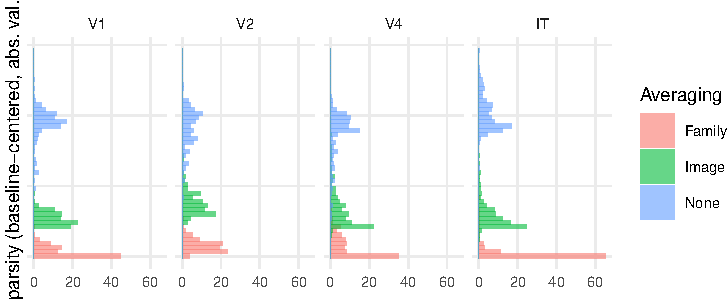
\includegraphics[keepaspectratio]{20261007_files/figure-pdf/fig-sparsity_avgs-1.pdf}}

}

\caption{\label{fig-sparsity_avgs}Changes in regional sparsity
distributions based on whether stimuli are not averaged (None), averaged
over repetitions of the same image (Image), or averaged over families
(Family). More averaging shifts the distribution left.}

\end{figure}%

\begin{figure}

\centering{

\pandocbounded{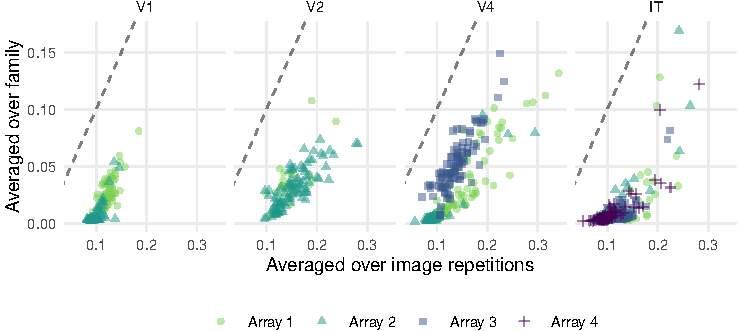
\includegraphics[keepaspectratio]{20261007_files/figure-pdf/fig-sparsity_fam_vs_img-1.pdf}}

}

\caption{\label{fig-sparsity_fam_vs_img}Changes in regional sparsity
distributions based on whether stimuli are averaed over family or
averaged over repetitions of the same image.}

\end{figure}%

\subsection{Sparsity measures generally
agree}\label{sparsity-measures-generally-agree}

The two approaches to sparsity generally agree, though IT is somewhat
less strongly correlated. Unless otherwise specified, results will
reflect the ratio of moments estimator, which is more common in
neuroscience.

\begin{itemize}
\tightlist
\item
  I haven't updated this with the averaging/baseline handling
\item
  Might be an addendum later
\end{itemize}

\subsection{Sparsities and reliability (split-half
correlation)}\label{sparsities-and-reliability-split-half-correlation}

The relationship between split-half reliability and sparsity is not
obvious (Figure~\ref{fig-corr_vs_sparsity}). The overall results do not
change when using Spearman-Brown corrected Pearson's
(Figure~\ref{fig-spearman_vs_sparsity}). In general, IT tends to show
higher lifetime sparsity for each site. Both IT and V1 show at least one
array with an apparent positive relationship.

\begin{figure}

\centering{

\pandocbounded{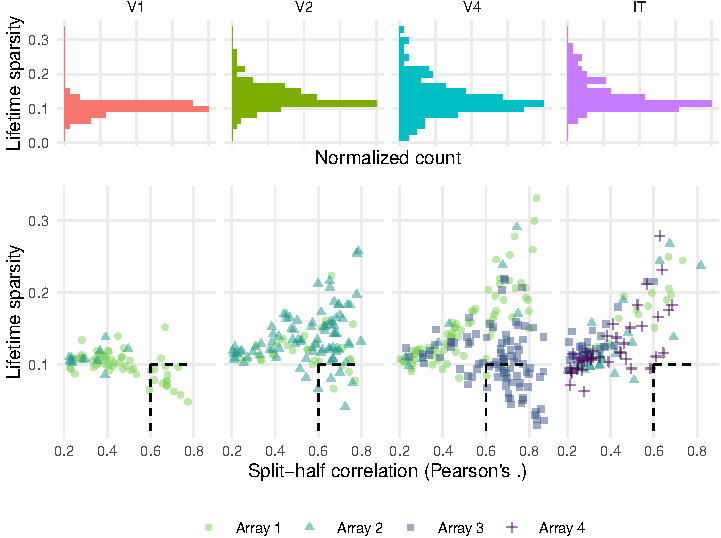
\includegraphics[keepaspectratio]{20261007_files/figure-pdf/fig-corr_vs_sparsity-1.pdf}}

}

\caption{\label{fig-corr_vs_sparsity}Scatter plot of sparsity and
split-half correlation for each site, separated by region. In general,
IT shows higher sparsity, though the correlation with reliability is not
obvious. Both V1 and IT show a cluster of low-reliability sites with a
wide distribution of clustering.}

\end{figure}%

\begin{figure}

\centering{

\pandocbounded{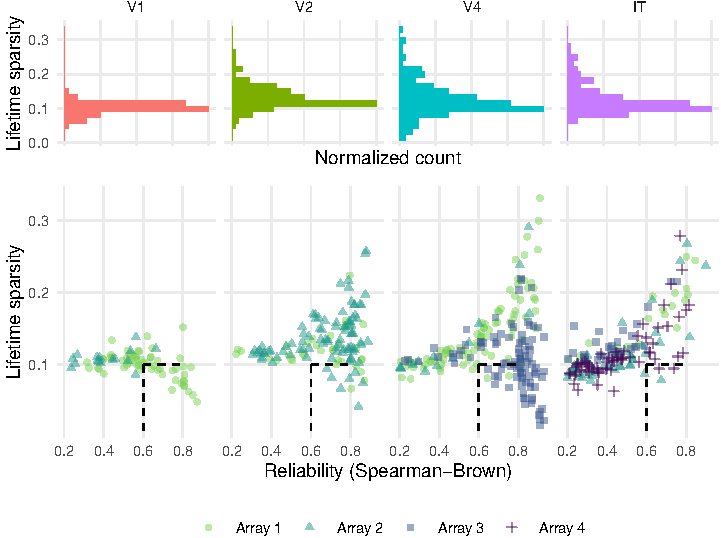
\includegraphics[keepaspectratio]{20261007_files/figure-pdf/fig-spearman_vs_sparsity-1.pdf}}

}

\caption{\label{fig-spearman_vs_sparsity}Scatter plot of sparsity and
Spearman-Brown corrected split-half correlation for each site, separated
by region. In general, IT shows higher sparsity, though the correlation
with reliability is not obvious. Both V1 and IT show a cluster of
low-reliability sites with a wide distribution of clustering.}

\end{figure}%

\section{Big question}\label{big-question}

So far, there are a couple of ``simple'' insights:

\begin{itemize}
\tightlist
\item
  In IT, sparsity tends to be more positively correlated with
  reliability.
\item
  In IT, responses tend to be sparse on the image level, so taking
  averages over the family kills the sparsity.
\item
  Thus, there's a fairly clean link between why a reliability cutoff
  over more images penalizes IT more than other reasons.
\end{itemize}




\end{document}
